
% The \phantomsection command is needed to create a link to a place in the document that is not a
% figure, equation, table, section, subsection, chapter, etc.
% https://tex.stackexchange.com/questions/44088/when-do-i-need-to-invoke-phantomsection
\phantomsection

% Multiple-language document - babel - selectlanguage vs begin/end{otherlanguage}
% https://tex.stackexchange.com/questions/36526/multiple-language-document-babel-selectlanguage-vs-begin-endotherlanguage
\begin{otherlanguage*}{brazil}

\chapter{Desenvolvimento}

Nesta seção, será abordada a LTI do Beecrowd, que simplifica a integração entre o Moodle e a plataforma Beecrowd. Serão apresentados também os detalhes da implementação da aplicação web do sistema especialista, desenvolvida para auxiliar professores e alunos no esclarecimento de dúvidas recorrentes sobre as questões do Beecrowd, facilitando a adaptação de ambos ao uso da plataforma.

\section{LTI BEECROWD}

Com a disponibilização de uma ferramenta LTI pelo Beecrowd, visando facilitar sua integração com o Moodle, foi elaborado um manual detalhado para orientar o administrador do Moodle na configuração dessa LTI (Apêndice A).

Para configurar uma LTI externa, o administrador deve acessar "Administração do site", selecionar "Plugins" e, em "Módulos de atividade", escolher "Ferramenta externa" e clicar em "Gerenciar ferramentas". Em seguida, deve clicar em "Configurar uma ferramenta manualmente" e preencher os campos conforme as instruções especificadas no Manual de Configuração da LTI Beecrowd no Moodle (Apêndice A). Após a configuração, será possível visualizar os detalhes da ferramenta, os quais deverão ser enviados ao Beecrowd para estabelecer a comunicação entre as plataformas.

Além disso, foi desenvolvido um manual de uso da LTI Beecrowd (Apêndice B), direcionado aos professores que desejam utilizar o Beecrowd como suporte educacional em sala de aula. Esse manual instrui os docentes sobre como criar uma atividade do Beecrowd no Moodle, orientar o acesso dos estudantes e transferir as notas obtidas no Beecrowd para o Moodle.

Após seguir o guia do Manual de Uso da LTI Beecrowd (Apêndice B), duas atividades ficam disponíveis na página do curso, apresentadas como "botões" visuais. A primeira atividade, que é ocultada para os estudantes (Imagem 23), permite ao professor acessar o Beecrowd Academic (Imagem 24) para configurar disciplinas, criar listas de exercícios para os alunos e enviar as notas para o Moodle.

\begin{figure}[H]
    \centering
            \caption{Atividade para o professor acessar o Beecrowd Academic}
            \label{fig:ModeloConceitual}
        
\includegraphics[scale=0.35]{pictures/apendices/apendice_b_5.png}
        \fonte{Produzido pela autora.}
\end{figure}

\begin{figure}[H]
    \centering
            \caption{Beecrowd Academic}
            \label{fig:ModeloConceitual}
        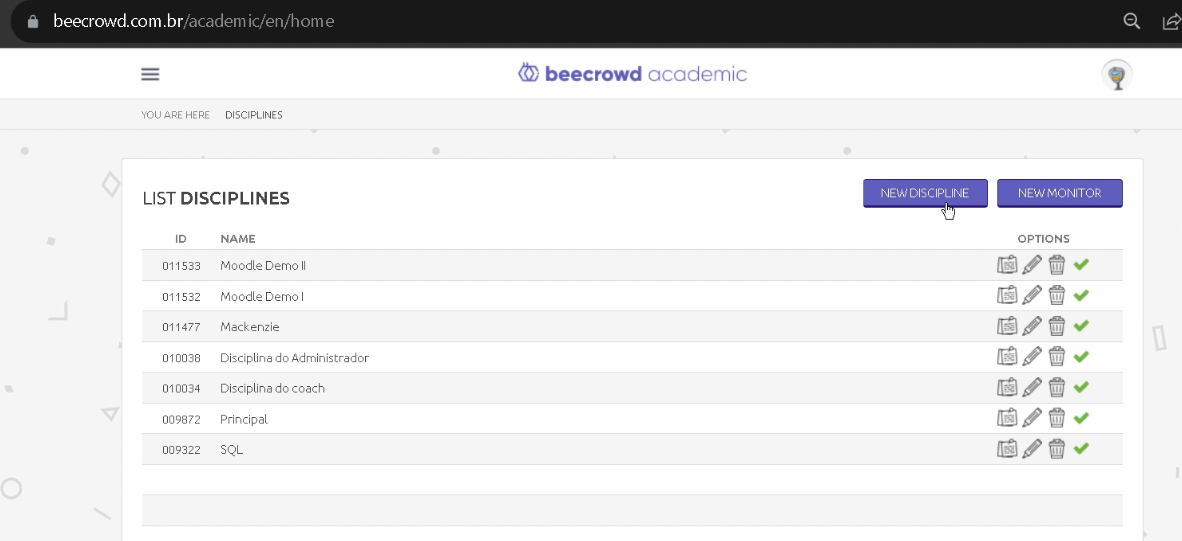
\includegraphics[scale=0.38]{pictures/desenvolvimento/lti_beecrowd_academic.png}
        \fonte{Produzido pela autora.}
\end{figure}

A segunda atividade, acessível aos estudantes (Imagem 25), redireciona-os diretamente para a página no Beecrowd da lista de exercícios criada pelo professor (Imagem 26), sem necessidade de cadastro ou login. Assim, os estudantes podem resolver as atividades diretamente a partir dessa página. Esse botão também permite ao professor acessar a lista de exercícios criada, podendo verificar o progresso dos alunos, as tentativas realizadas e, quando desejado, enviar as notas para o Moodle.

\begin{figure}[H]
    \centering
            \caption{Atividade para o aluno acessar o Beecrowd}
            \label{fig:ModeloConceitual}
        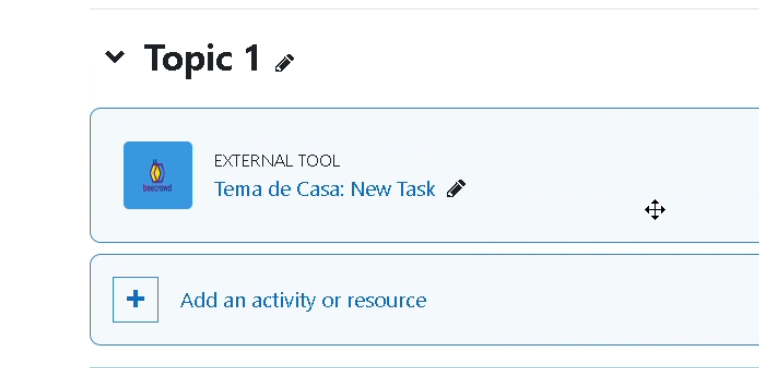
\includegraphics[scale=0.4]{pictures/desenvolvimento/lti_tarefa.png}
        \fonte{Produzido pela autora.}
\end{figure}

\begin{figure}[H]
    \centering
            \caption{Beecrowd do aluno}
            \label{fig:ModeloConceitual}
        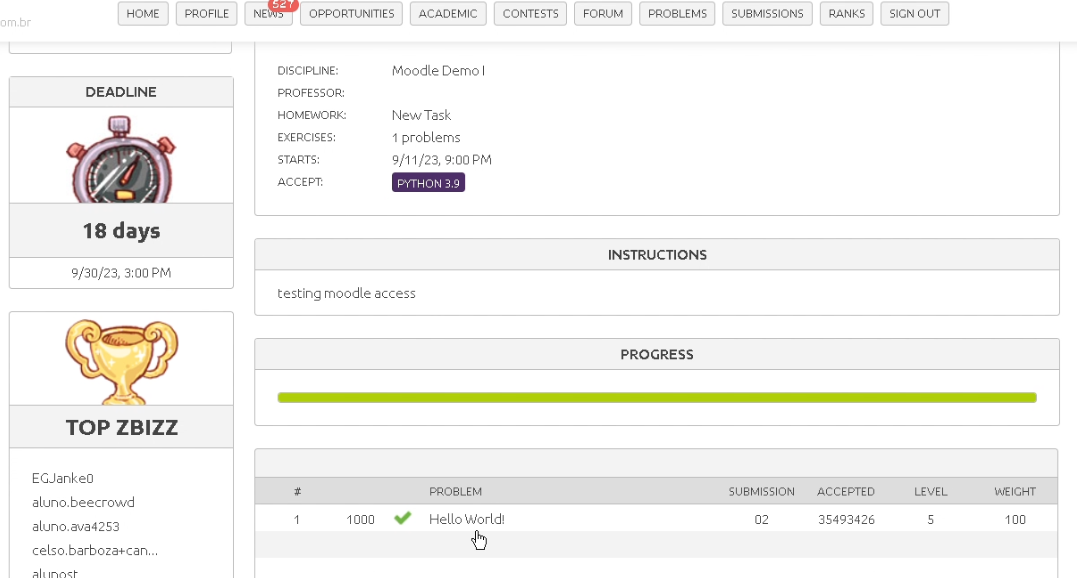
\includegraphics[scale=0.4]{pictures/desenvolvimento/lti_beecrowd_aluno.png}
        \fonte{Produzido pela autora.}
\end{figure}

\section{SISTEMA ESPECIALISTA WEB}

O objetivo do sistema especialista é oferecer suporte na resolução de dúvidas recorrentes dos estudantes em relação a questões do Beecrowd. A proposta é desenvolver uma aplicação acessível aos alunos via navegador, com um sistema de chat onde o aluno pode informar a questão sobre a qual necessita orientação. O sistema, então, conduz o aluno por meio de perguntas binárias (sim ou não) e, conforme as respostas, fornece dicas relevantes relacionadas ao exercício em questão.

Para viabilizar essa funcionalidade, o sistema especialista será estruturado com um conjunto de dados contendo perguntas direcionadas aos alunos e respostas predefinidas que orientam o aluno na resolução das atividades específicas da disciplina. Em disciplinas como Programação Orientada a Objetos I, onde as listas de exercícios frequentemente incluem questões já utilizadas em semestres anteriores, observa-se uma repetição de problemas e, consequentemente, de dúvidas recorrentes dos alunos.

Assim, a primeira etapa deste trabalho consistiu na coleta de dados sobre as questões, visando identificar e catalogar as dúvidas mais comuns.

\subsection{\textbf{Coleta de Dados}}

Nesta fase, foram realizadas duas coletas de dados: uma com dicas de resolução fornecidas pelo professor para uma lista de exercícios, e outra com as dúvidas dos alunos sobre o uso de listas em Python, com foco em questões específicas.

Na primeira coleta, professor da disciplina de Programação Orientada a Objetos I, da Universidade Federal de Santa Catarina (UFSC), forneceu dicas de resoluções para cada questão de uma lista de exercícios que ainda não tinha sido repassada aos alunos, com o objetivo de avaliar a utilidade da aplicação após ela ser desenvolvida. Assim, quando os alunos fossem resolver a lista de exercícios, poderiam testar a aplicação para ser sua eficácia. As questões abordadas, que receberam as dicas de solução, incluem: 1261, 1281, 1430, 1449, 1483, 1763, 1991, 1953, 2091, 2482, 2492, 2654, 2949 e 2987.

Na segunda coleta, foram registradas as dúvidas dos alunos da disciplina de Programação Orientada a Objetos I, da UFSC, coletadas no dia 30 de outubro de 2024. Nessa data, os alunos estavam trabalhando em uma lista de exercícios sobre o uso de listas em Python. As questões abordadas incluíram os problemas de números 1187, 1435, 1715, 2436, 1383, 1184, 1181 e 1185. Um aspecto notável foi que, durante essa mesma aula, quatro alunos apresentaram a mesma dúvida em relação à questão 1435, especificamente perguntando: "Como resolvo essa questão?"

Durante as 2h30 de aula, a questão 1435 foi a que suscitou o maior número de dúvidas entre os estudantes. Em uma turma de 26 alunos – embora nem todos tenham alcançado essa questão no tempo da aula –, quatro solicitaram uma explicação geral sobre a abordagem para resolvê-la, enquanto dois buscaram orientação sobre a conversão dessa abordagem para o código. Adicionalmente, três alunos enfrentaram o erro "Presentation Error" e um aluno recebeu o erro "Run-time Error".

As dúvidas em relação à questão 1181 refletiram dificuldades comuns no uso de laços de repetição e na manipulação de matrizes. Muitos estudantes não obtinham a resposta correta, mesmo com uma solução aparentemente desenvolvida, devido à confusão na seleção dos elementos da matriz, com erros ao iterar pelas linhas em vez das colunas. Os alunos também enfrentaram dificuldades na estruturação do laço de repetição, especialmente ao calcular a soma dos elementos de uma linha específica e ao determinar o divisor correto para o cálculo da média. Problemas de formatação, que resultaram no erro "Presentation Error", também foram recorrentes, sendo necessário ajustar a saída para uma casa decimal com '%.1f'.

Na questão 1184, as dificuldades estavam relacionadas à estruturação do laço de repetição para percorrer corretamente os elementos abaixo da diagonal principal da matriz. Os alunos foram orientados a usar um laço duplo, com a sequência correta de for i in range(0, 12) e for j in range(0, i). Além disso, houve dúvidas sobre a exclusão dos elementos da diagonal principal, que não deveriam ser somados. Como na questão 1181, os alunos enfrentaram dificuldades de formatação, com orientações para ajustar a saída utilizando '%.1f' para obter uma casa decimal.

As dúvidas relativas à questão 1185 envolveram a manipulação de elementos acima da diagonal secundária da matriz, com os alunos sendo orientados a percorrer as linhas até o último índice da coluna, subtraindo o número da linha. A configuração correta dos laços de repetição foi outra dúvida comum, com muitos alunos invertendo os laços, o que afetou os resultados. A correção do divisor para o cálculo da média e os problemas de formatação também foram pontos críticos, com instruções para usar '%.1f' na saída.

A questão 1187 gerou dúvidas relacionadas aos laços de repetição necessários para somar os elementos da matriz, com os alunos questionando sobre o ajuste dos índices para evitar a soma dos elementos das diagonais. Também surgiram dúvidas sobre como os laços percorriam as linhas e colunas para formar a região triangular desejada, além de questionamentos sobre a lógica para calcular a média e evitar erros de divisão.

A questão 1383, sobre as regras do Sudoku, suscitou dúvidas sobre como validar se uma solução estava correta, além de dificuldades na transformação da lógica para código. A orientação dada foi garantir a não repetição de números em cada linha, coluna, e bloco 3x3, com orientações sobre o uso de depuração com o udebug e Thonny.

A questão 1715 gerou dúvidas sobre a multiplicação dos elementos das linhas para identificar jogadores que marcaram gols em todas as partidas. Os alunos tiveram dificuldades em entender como aplicar esse método corretamente e como garantir que o contador fosse atualizado. A depuração no udebug e Thonny foi útil para a maioria dos alunos, que ajustaram seus códigos após o feedback.

Por fim, a questão 2465 também gerou dúvidas em relação ao uso do comando while True para verificar os vizinhos da matriz. A principal dificuldade foi evitar que o robô retornasse à posição anterior após avançar para um vizinho com valor '1', sendo sugerido que a posição fosse marcada como zero antes de seguir para o próximo vizinho. As orientações permitiram que os alunos avançassem na resolução do problema, superando as dificuldades iniciais.

\subsection{\textbf{Tecnologias Usadas}}

\subsubsection{\textbf{\textit{Prolog e SWI-Prolog}}}

Para o desenvolvimento do backend da aplicação, utilizou-se a linguagem Prolog, com o auxílio da implementação SWI-Prolog. O SWI-Prolog é uma versão amplamente utilizada do Prolog, que inclui uma série de bibliotecas essenciais para a manipulação de requisições HTTP e dados JSON, como http/thread\_httpd, http/http\_dispatch, http/json, http/http\_session, entre outras. Essas bibliotecas permitem a configuração de um servidor HTTP para o processamento de requisições web e a manipulação de dados JSON. Além disso, elas possibilitam o gerenciamento de sessões, o que viabiliza a integração com aplicações externas e permite o uso simultâneo da aplicação por diferentes usuários \cite{swiprologhttp}.

\subsubsection{\textbf{\textit{API REST}}}

O servidor definiu os endpoints HTTP (/server e /diagnosis) para o recebimento de requisições POST e GET, permitindo a interação com o backend por meio de uma arquitetura baseada em REST. 

O termo REST (Representational State Transfer) é um estilo de comunicação baseado em padrões e protocolos da web, como HTTP, que permite a troca de dados entre sistemas de forma escalável e eficiente. Nesse modelo, as requisições são realizadas utilizando os métodos HTTP padrão (como GET, POST, PUT e DELETE), facilitando a comunicação entre sistemas de maneira eficiente e escalável \cite{whatisrest}.

\subsubsection{\textbf{\textit{JSON}}}

JSON (JavaScript Object Notation) é um formato leve e baseado em texto para intercâmbio de dados, independente de linguagem de programação. Derivado do padrão ECMAScript, o JSON define um conjunto simples de regras de formatação para a representação portátil de dados estruturados. Ele busca remover inconsistências com outras especificações e oferece orientações para melhorar a interoperabilidade entre sistemas \cite{whatisjson}.

A biblioteca http/http\_json do SWI-Prolog é utilizada para formatar as respostas no formato JSON, possibilitando que o backend envie dados estruturados para o frontend em um formato amplamente compatível com diversos frameworks web, incluindo o React. Essa abordagem facilita a troca de informações entre o servidor e a interface do usuário, garantindo a interoperabilidade e a eficiência na comunicação entre as camadas da aplicação.

\subsubsection{\textbf{\textit{HTTP e CORS}}}

CORS (Cross-Origin Resource Sharing) é um mecanismo que permite que requisições do lado do cliente acessem recursos de origens diferentes. Ele define algoritmos que possibilitam que uma API faça requisições a recursos de outra origem, controlando o acesso por meio de cabeçalhos de resposta, como o \textit{Access-Control-Allow-Origin} \cite{whatiscors}.

HTTP (Hypertext Transfer Protocol) é um protocolo de aplicação para sistemas distribuídos e colaborativos de informações hipermídia. É um protocolo genérico e sem estado, utilizado em diversas tarefas além do hipertexto, como servidores de nomes e sistemas de gerenciamento de objetos distribuídos. O HTTP permite a negociação e tipificação da representação dos dados, possibilitando a construção de sistemas independentes dos dados transferidos \cite{whatishttp}.

As bibliotecas http/thread\_httpd, http/http\_dispatch e http/http\_cors, do SWI-Prolog, configuram um servidor HTTP básico, sendo responsáveis pelo tratamento de requisições e respostas. Elas também gerenciam as permissões de CORS, permitindo que o frontend (React) acesse o backend Prolog, mesmo quando este está hospedado em uma origem diferente.

\subsubsection{\textbf{\textit{Sessões HTTP}}}

Uma sessão HTTP é mantida por meio do uso de cookies, que são pequenos arquivos de dados armazenados nos agentes de usuário (como navegadores) pelos servidores HTTP. Os cabeçalhos Cookie e Set-Cookie permitem que os servidores mantenham o estado de uma sessão, mesmo em um protocolo essencialmente sem estado como o HTTP. Isso significa que, através das sessões, os servidores podem armazenar informações sobre o usuário, como preferências ou dados de autenticação, e usá-las em requisições subsequentes, garantindo uma experiência contínua. Embora os cookies tenham questões históricas relacionadas à segurança e privacidade, os cabeçalhos Cookie e Set-Cookie são amplamente utilizados para gerenciar sessões de usuário, permitindo, por exemplo, o login persistente em sites ou a manutenção de um carrinho de compras em uma loja online \cite{whatissession}.

A biblioteca http/http\_session do SWI-Prolog possibilita o gerenciamento de sessões de usuário, permitindo o armazenamento de variáveis de sessão, como questionNumber e answers. Esse recurso viabiliza a persistência de informações entre requisições subsequentes de um mesmo usuário, assegurando a continuidade do estado da aplicação ao longo da interação.

\subsubsection{\textbf{\textit{React e Typescript (Frontend)}}}

O frontend foi feito em React\footnote{\url{https://react.dev/}} e Typescript\footnote{\url{https://www.typescriptlang.org/}}, interagindo com o backend por meio de requisições HTTP, acessando endpoints para enviar as respostas do usuário e buscar o resultado final da questão.

React é uma biblioteca para a construção de interfaces de usuário, tanto para a web quanto para aplicativos nativos. Ela permite criar interfaces a partir de unidades individuais chamadas componentes, que podem ser reutilizados e combinados para formar interfaces complexas e interativas. Cada componente em React gerencia seu próprio estado e pode ser renderizado de forma eficiente conforme as mudanças nos dados, facilitando o desenvolvimento de aplicações dinâmicas e de fácil manutenção. React pode ser utilizado com outras linguagens que compilam para JavaScript\footnote{\url{https://www.javascript.com/}}, como TypeScript.

TypeScript é uma linguagem de programação que é um superconjunto do JavaScript, adicionando tipagem estática. Isso permite que os desenvolvedores definam tipos para variáveis e funções, ajudando a identificar erros antes da execução do código. TypeScript melhora a manutenção e segurança do código, especialmente em projetos grandes, e é amplamente utilizado com frameworks como React para criar aplicações mais escaláveis e robustas.

\section{ARQUITETURA DE SOFTWARE}

A aplicação propõe uma interação dinâmica em que o usuário, ao informar o número da questão sobre a qual deseja obter orientações, inicia um diálogo com o sistema de chat. O chat responde com perguntas específicas para compreender melhor as necessidades do usuário, permitindo direcionar as orientações de forma mais precisa. Conforme o usuário responde com "sim" ou "não" a cada pergunta, o sistema adapta as próximas questões e sugestões, guiando-o progressivamente até fornecer uma orientação final ajustada ao contexto das respostas acumuladas.

A Figura 27 apresenta o diagrama de atividades que detalha o fluxo de interação entre o usuário e o chat da aplicação. Após informar o número da questão sobre a qual deseja obter orientações, o usuário recebe uma pergunta inicial, respondendo com "sim" ou "não". Se houver mais perguntas, o chat continua a apresentá-las até que todas sejam respondidas, conduzindo o usuário a uma orientação final baseada nas respostas acumuladas. Ao final, o usuário pode iniciar o processo novamente com outro número de questão ou com o mesmo, caso deseje explorar outras sugestões e perguntas relacionadas.

\begin{figure}[h!]
    \centering
            \caption{Diagrama de Atividades do Usuário da Aplicação}
            \label{fig:ModeloConceitual}
        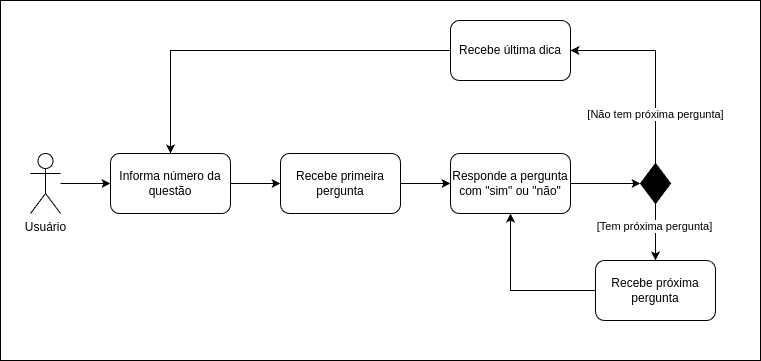
\includegraphics[scale=0.6]{pictures/atividade1.png}
        \fonte{Produzido pela autora.}
\end{figure}

A Figura 28 representa a estrutura da aplicação, mostrando a interação entre o frontend e o backend através de requisições. No frontend, o arquivo ActionProvider gerencia as mensagens enviadas pelo usuário no chat, processando tanto o número da questão informada (Imagem 29) quanto as respostas de "sim" ou "não" (Imagem 30). Por meio dessas requisições, o frontend envia esses dados ao backend, que, em resposta, fornece perguntas e dicas relacionadas à questão solicitada. Caso o usuário peça uma nova dica e o backend não tenha mais sugestões para aquela questão, ele notifica o frontend. Em resposta, o frontend faz uma nova requisição ao backend para obter a orientação final da questão, que é então apresentada ao usuário.

\begin{figure}[h!]
    \centering
            \caption{Arquitetura da Aplicação do Sistema Especialista}
            \label{fig:ModeloConceitual}
        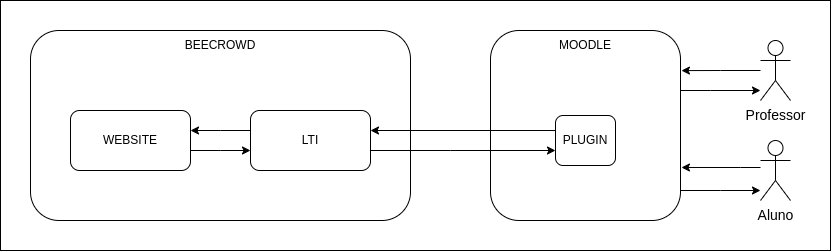
\includegraphics[scale=0.6]{pictures/arquitetura.png}
        \fonte{Produzido pela autora.}
\end{figure}

\begin{lstlisting}
const handleFirstMessage = async (questionNumber?: string) => {
    const body = new URLSearchParams({ questionNumber: questionNumber?.toString() || '' });
    const data = await fetchData("http://localhost:6358/server", body);
    let additionalMessages: {
        messages: {
        message: string;
        type: string;
        id: number;
        loading?: boolean;
        widget?: string | undefined;
        delay?: number | undefined;
        payload?: any;
        }[];
    }[] = [];

    await handleMessageResponse(data, additionalMessages);    
    
    setState((prev: {
        messages: {
        message: string;
        type: string;
        id: number;
        loading?: boolean;
        widget?: string | undefined;
        delay?: number | undefined;
        payload?: any;
        }[];
    }) => ({
        ...prev,
        messages: [...prev.messages, ...additionalMessages],
    }));
};
\end{lstlisting}

\begin{lstlisting}
const handleFirstMessage = async (questionNumber?: string) => {
    const body = new URLSearchParams({ questionNumber: questionNumber?.toString() || '' });
    const data = await fetchData("http://localhost:6358/server", body);
    let additionalMessages: {
        messages: {
        message: string;
        type: string;
        id: number;
        loading?: boolean;
        widget?: string | undefined;
        delay?: number | undefined;
        payload?: any;
        }[];
    }[] = [];

    await handleMessageResponse(data, additionalMessages);    
    
    setState((prev: {
        messages: {
        message: string;
        type: string;
        id: number;
        loading?: boolean;
        widget?: string | undefined;
        delay?: number | undefined;
        payload?: any;
        }[];
    }) => ({
        ...prev,
        messages: [...prev.messages, ...additionalMessages],
    }));
};
\end{lstlisting}


\begin{lstlisting}
const handleMessageResponse = async (data: any, additionalMessages: any[]) => {
    const { question, result, error } = data;

    if (error) {
        additionalMessages.push(createChatBotMessage(error, {}));
    } else if (question) {
        /* Exemplo de atualização do messages-slice, caso precise no futuro
        dispatch(addQuestion(question));
        setTimeout(() => dispatch(startCount(question.length)), 5000);
        */

        const lines = question.split('\n');
        lines.forEach((line: string, index: number) => {
            if (line.trim() !== "") {
                const isLastLine = index === lines.length - 1;
                const message = isLastLine
                    ? createChatBotMessage(line, { widget: "yesNo" })
                    : createChatBotMessage(line, {});

                additionalMessages.push(message);
            }
        });

    } else if (result || error) {
        additionalMessages.push(createChatBotMessage(error || result || "Mensagem inválida recebida.", {}));
        const diagnosis = await handleEnd();
        if (diagnosis) additionalMessages.push(createChatBotMessage(diagnosis, {}));
        additionalMessages.push(createChatBotMessage("Gostaria de tirar dúvidas novamente?", { widget: "exerciseDropdown" }));
    }
};
\end{lstlisting}


\begin{lstlisting}
const fetchData = async (url: string, body: URLSearchParams) => {
    try {
        const response = await fetch(url, {
        method: "POST",
        headers: { 'Content-Type': 'application/x-www-form-urlencoded;charset=UTF-8' },
        credentials: 'include',
        body,
        });

        if (response.status !== 200) throw new Error("Erro ao consultar o backend.");

        return await response.json();
    } catch (error) {
        return { error: "Erro ao consultar o backend." };
    }
};
\end{lstlisting}


Também observa-se que o \textit{backend} é composto pelo arquivo principal \textit{server.pl} e por arquivos de questões nomeados no formato \textit{questao\_\{numeroDaQuestão\}.pl}, contendo as dicas para cada questão específica. Por exemplo, o arquivo \textit{questao\_1234.pl} armazena as dicas da questão 1234 do Beecrowd. O \textit{server.pl} inicia um servidor HTTP, configurando rotas para processar requisições e habilitando CORS para aceitar conexões da porta do \textit{frontend}. Ele recebe requisições \textit{POST} para iniciar ou continuar uma questão, associando cada sessão ao usuário que fez a requisição, além de aceitar requisições \textit{GET} para obter o diagnóstico final com base nas respostas acumuladas.

Os arquivos de questões são carregados dinamicamente no \textit{server.pl} com base no número da questão recebido nas requisições \textit{POST}, e as informações fornecidas pelo usuário — como número da questão e respostas — são armazenadas na sessão do usuário para garantir a continuidade da interação. Se o usuário alterna para uma nova questão, por exemplo, a questão Y, o \textit{backend} carrega o arquivo \textit{questao\_Y.pl} e passa a conduzir a interação de acordo com suas informações. No final do processo, ao esgotarem-se as perguntas para o usuário, o \textit{backend} notifica o \textit{frontend}, que solicita então o resultado final, completando a interação com a entrega da orientação ao usuário.

\section{REQUISITOS DA APLICAÇÃO}

\subsection{Regras de Negócio}

\textbf{RG1 – Importação de Notas:} O sistema deve importar as notas do Beecrowd para o Moodle apenas para disciplinas e tarefas previamente associadas, evitando importações não autorizadas;

\vspace{12pt}

\textbf{RG2 – Cadastro Automático de Alunos:} Alunos podem se cadastrar automaticamente no Beecrowd pelo Moodle somente se estiverem matriculados nas disciplinas habilitadas para uso do Beecrowd;

\vspace{12pt}

\textbf{RG3 – Criação Automática de Disciplina:} A criação automática de disciplinas no Beecrowd ao habilitar o uso deve seguir uma estrutura de nomenclatura padronizada para facilitar a identificação;

\vspace{12pt}

\textbf{RG4 – Visualização de Submissões:} A visualização de submissões de alunos no Beecrowd pelo Moodle só é permitida para professores associados às disciplinas correspondentes;

\vspace{12pt}

\textbf{RG5 – Submissão de Solução:} Alunos só podem submeter soluções no Beecrowd via Moodle para as listas de exercícios ativas e dentro dos prazos estabelecidos;

\vspace{12pt}

\textbf{RG5 – Acesso às Listas de Exercícios:} O acesso às listas de exercícios e questões no Moodle está disponível apenas durante o período em que a disciplina está em andamento.

\vspace{12pt}

\subsection{Requisitos Não Funcionais}

\textbf{RNF01 – Linguagem de Programação e Tecnologias Front-end:} O plugin deve ser desenvolvido utilizando a linguagem de programação PHP para a lógica de back-end e HTML, CSS e Javascript para adaptar o frontend;

\vspace{12pt}

\textbf{RNF02 – Interface Responsiva:} A interface do usuário deve ser responsiva e seguir as melhores práticas de design para garantir uma experiência do usuário consistente;

\vspace{12pt}

\textbf{RNF03 – Estrutura de Diretórios e Arquivos:} O código do plugin deve seguir a estrutura de diretórios e arquivos especificada na seção "Fundamentos Teóricos", na subseção "Plugin do Moodle";

\vspace{12pt}

\textbf{RNF04 – Padrões de Desenvolvimento:} O código do plugin deve aderir aos padrões de codificação estabelecidos para o desenvolvimento de plugins no ambiente Moodle, incluindo boas práticas de programação, documentação e modularidade para assegurar a qualidade e manutenibilidade do código;

\vspace{12pt}

\textbf{RNF05 – Diagrama UML:} A implementação do plugin deve seguir as especificações detalhadas no diagrama UML fornecido, garantindo que a estrutura e os relacionamentos definidos sejam fielmente reproduzidos no sistema;

\vspace{12pt}

\textbf{RNF06 – Integração com LTI (Learning Tools Interoperability):} O plugin deve ser desenvolvido com integração compatível com o padrão LTI, assegurando interoperabilidade eficaz com outras ferramentas educacionais que suportem esse padrão;

\vspace{12pt}

\textbf{RNF07 – Documentação do Plugin:} Deve ser fornecida uma documentação completa e clara, incluindo README, CHANGES e outros arquivos necessários, facilitando a instalação, configuração e utilização do plugin por parte dos administradores e usuários;

\vspace{12pt}

\textbf{RNF08 – Compatibilidade com Versões do Moodle:} O plugin deve ser compatível com as versões específicas do Moodle, conforme indicado nas diretrizes de suporte e requisitos do sistema, para garantir a funcionalidade em ambientes Moodle diversos;

\vspace{12pt}

\textbf{RNF09 – Segurança:} O plugin deve incorporar medidas de segurança adequadas para proteger contra vulnerabilidades conhecidas;

\vspace{12pt}

\textbf{RNF10 – Desempenho:} O plugin deve ser otimizado para garantir desempenho eficiente, minimizando tempo de carregamento e consumo de recursos do sistema, proporcionando uma experiência rápida e responsiva;

\vspace{12pt}

\textbf{RNF11 – Compatibilidade:} O plugin deve ser compatível com os principais navegadores (Chrome, Firefox, Safari) e dispositivos (desktop, tablet, mobile) para garantir uma experiência consistente.

\subsection{Requisitos Funcionais}

\textbf{RF01 – Importação de Notas do Beecrowd para o Moodle:} O sistema deve permitir a importação automática das notas dos alunos no Beecrowd para o Moodle;

\vspace{12pt}

\textbf{RF02 – Cadastro Automático no Beecrowd via Moodle:} Os alunos devem ter a opção de realizar o cadastro automaticamente no Beecrowd por meio do Moodle;

\vspace{12pt}

\textbf{RF03 – Criação Automática de Disciplina no Beecrowd:} Ao habilitar o uso do Beecrowd no Moodle para uma disciplina, o sistema deve criar automaticamente a correspondente disciplina no Beecrowd;

\vspace{12pt}

\textbf{RF04 – Visualização de Submissões no Beecrowd pelo Moodle:} Os professores devem ser capazes de visualizar as submissões dos alunos no Beecrowd, juntamente com os feedbacks fornecidos pelo Beecrowd, diretamente no Moodle;

\vspace{12pt}

\textbf{RF05 – Criação de Listas e Competições no Beecrowd pelo Moodle:} Professores devem poder criar listas de exercícios e competições no Beecrowd diretamente através do ambiente Moodle;

\vspace{12pt}

\textbf{RF06 – Submissão de Solução no Beecrowd via Moodle:} Alunos devem ser capazes de submeter suas soluções para as listas de exercícios do Beecrowd diretamente através do Moodle;

\vspace{12pt}

\textbf{RF07 – Acompanhamento do Progresso no Beecrowd pelo Moodle:} Professores devem conseguir visualizar o progresso de cada aluno, tanto de forma geral na disciplina quanto em relação a cada lista de exercícios, no Beecrowd, pelo Moodle;

\vspace{12pt}

\textbf{RF08 – Acompanhamento do Próprio Progresso pelo Aluno:} Alunos devem poder visualizar seu próprio progresso geral na disciplina, assim como o desempenho em cada lista de exercícios e em cada exercício específico, no Beecrowd, pelo Moodle;

\vspace{12pt}

\textbf{RF09 – Acesso às Listas de Exercícios e Questões no Moodle:} Alunos e professores devem conseguir abrir as listas de exercícios do Beecrowd, incluindo o acesso aos enunciados das questões, diretamente no Moodle;

\vspace{12pt}

\textbf{RF10 – Definição de Linguagem de Programação no Moodle:} Professores devem poder definir a linguagem de programação para submissão das questões no Beecrowd, diretamente no Moodle, a fim de minimizar erros na seleção de versões inadequadas do Python;

\vspace{12pt}

\textbf{RF11 – Visualização do Feedback de cada submissão de exercício do Beecrowd pelo Moodle:} Deve ser possível ao aluno visualizar o feedback do Beecrowd para cada submissão de exercício diretamente pelo Moodle.

\end{otherlanguage*}

